\documentclass[10pt]{beamer}

\mode<presentation> 
{
  \usetheme{Diku}
  \beamertemplatenavigationsymbolsempty
  \setbeamercovered{invisible}
%  \setbeamercovered{transparent}
}


% { \usetheme[nat,dogma]{Frederiksberg} }
%{ \usetheme[nat]{Frederiksberg} }

% \usepackage[danish]{babel}
\usepackage[latin1]{inputenc}
\usepackage{times,pslatex}
\usepackage[T1]{fontenc}
\usepackage[english]{babel}
\usepackage{hyperref}

\usepackage{multimedia}
\usepackage{francois-preamble}
\usepackage{multirow}
% \usepackage{multimedia}


\newcommand{\cc}{{c\!\!,}}
\newcommand{\degr}[1]{{{#1}^\circ}}
\DeclareMathOperator{\idf}{idf}

\title{Content Based Image Retrieval}

\author[S. Olsen] % (optional, use only with lots of authors)
{S�ren I. Olsen}
% Copied from Francois Lauze

\institute[DIKU] % (optional, but mostly needed)
{
  Department of Computer Science\\
  University of Copenhagen
}

\date[2014 B2] % (optional, should be abbreviation of conference name)
% {Research Presentation, Diku 2006}

% Insert page numbers
\pagenumbering{arabic}
\setbeamertemplate{footline}{\hspace{5pt}\insertpagenumber\vspace{10pt}}

\definecolor{gold}{rgb}{0.95,0.83,0.0}
\definecolor{orange}{rgb}{0.95,0.7,0.0}
% \definecolor{backblue}{rgb}{0.93,0.94,0.99}
\definecolor{backblue}{rgb}{0.95,0.94,0.99}
\setbeamercolor*{background canvas}{bg=backblue} 



\newcommand{\myemph}[1]{{\color{blue}{#1}}}
\newcommand{\intrg}[1]{\int_{{#1}=-\infty}^\infty}
\newcommand{\intRR}{\int_{-\infty}^\infty}

\AtBeginSection[]
{
  \begin{frame}<beamer>{Outline}
    \tableofcontents[currentsection,currentsubsection]
  \end{frame}
}


\begin{document}
\maketitle

% would be cool with more images showing applications


%-------------------------------------------------------------------
%   Start slides
%-------------------------------------------------------------------

\begin{frame}
  \frametitle{Plan for today (and perhaps Wednesday)}
  \begin{itemize}
  \item How to query Image Databases \\[3mm]
  \item The idea of visual words, codebook, bag of visual words. \\[3mm]
  \item The two main ingredients for building visual words are image
    descriptors and data clustering.
  \end{itemize}
\end{frame}


\section{Introduction}

%-------------------------------------------------------------------
\begin{frame}
  \frametitle{Querying Images}
  \begin{itemize}
    \item Example from Google Images: Query using the word \texttt{apple}
    \begin{center}
      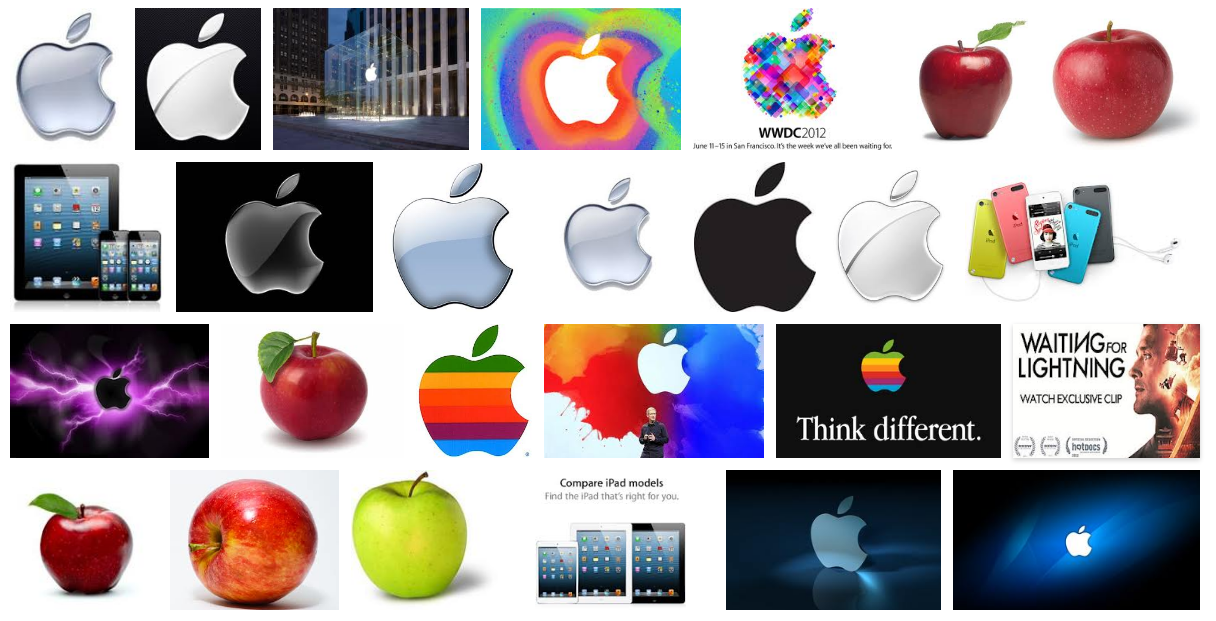
\includegraphics[width=0.8\textwidth]{FIGURES/GoogleAppleQuery}
    \end{center}
  \item Maybe not what expected! Try yourself and observe difference
    when using \texttt{apple} and \texttt{an apple}
  \end{itemize}
\end{frame}


%-------------------------------------------------------------------
\begin{frame}
  \begin{itemize}
  \item Simple textual description may fail. Reasons are multiple:\\[3mm]
    \begin{itemize}
    \item Language ambiguity ... \\[3mm]
    \item  Lack of proper image annotation ... \\[3mm]
    \item {\color{red}{Can you think of others?}}
    \end{itemize}
  \end{itemize}
\end{frame}


%-------------------------------------------------------------------
\begin{frame}
  \frametitle{Another approach}
  \begin{itemize}
  \item Replace simple textual description by content based analysis.  \\[5mm]
  \item {\color{red}{\bf Exercise:} What content?} \\
           Discuss for 2 minutes with your neighbor what might be good
           image features for CBIR \\[5mm]
  \pause
  \item Use for instance Intensity, color, texture, shape etc... in a
    global or local setting.
%   \item Find efficient ways to answer the question:\\
%     \emph{What makes an image of an apple resemble an image of an apple?}
  \end{itemize}
\end{frame}


%-------------------------------------------------------------------
\begin{frame}
  \frametitle{An Inspiration: Text Mining}
  \begin{center}
    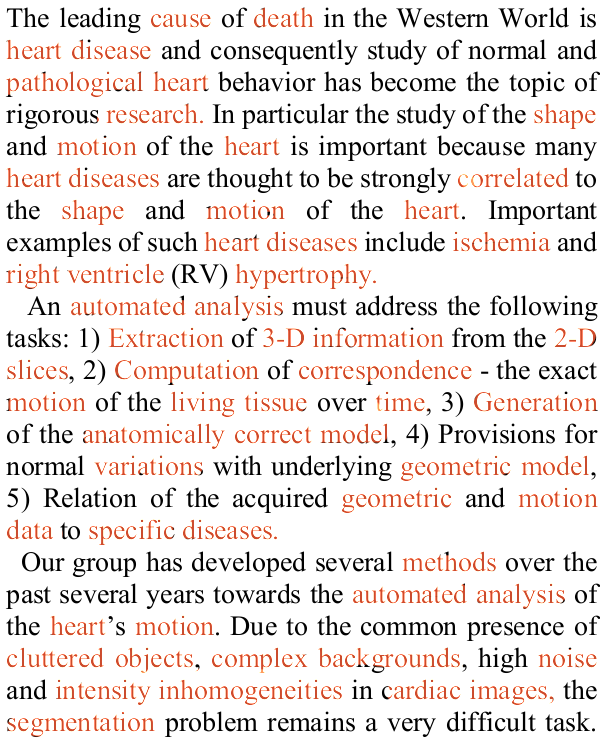
\includegraphics[width=0.5\textwidth,height=0.8\textheight]{FIGURES/ScreenshotMETAXAS}
      ~~
    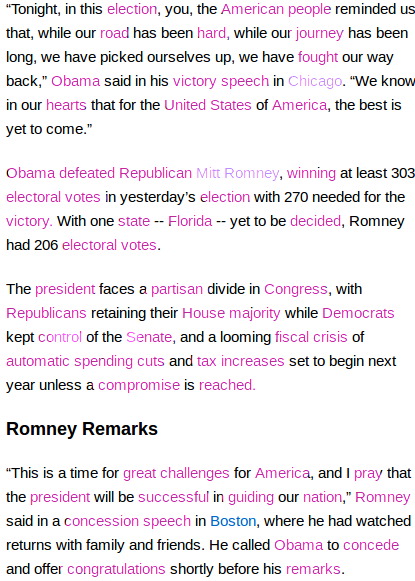
\includegraphics[width=0.5\textwidth,height=0.8\textheight]{FIGURES/ScreenshotBloomberg}
  \end{center}
\end{frame}


%-------------------------------------------------------------------
\begin{frame}
  \frametitle{Some statistics from these documents}
  Partial word count of the most frequent ones, eliminating very common ``the, and, of, is \dots''
  \vspace{-3mm}
  \begin{columns}
    \column{0.5\textwidth}
    \begin{center}
      Document 1
    \end{center}
    \vspace{-5mm}
    \begin{itemize}
    \item 7 times \textbf{heart}
    \item 4 times \textbf{disease(s)}
    \item 3 times \textbf{motion}
    \item 2 times \textbf{geometric}
    \item 2 times \textbf{shape}
    \item 2 times \textbf{model}
    \end{itemize}
    \column{0.5\textwidth}
    \begin{center}
      Document 2
    \end{center} 
    \vspace{-5mm}
    \begin{itemize}
    \item 3 times \textbf{elect(ion|oral)}
    \item 2 times \textbf{America(n)}
    \item 2 times \textbf{president}
    \item 2 times \textbf{speech}
    \item 2 times \textbf{state(s)}
    \item 1 time \textbf{heart}
    \end{itemize}
  \end{columns}
  ~\\
  \begin{itemize}
  \item Even discarding  grammatical structure, very different distributions.
  \item Some variation around a word were grouped ``disease|diseases'', ``election|electoral'', ``America|American''...
  \end{itemize}
\end{frame}


\section{Bag of Visual Words}
\label{sec:bovw}


%-------------------------------------------------------------------
\begin{frame}
  \frametitle{Visual Words}
  \begin{itemize}
  \item Visual words: what to choose?
    \begin{center}
      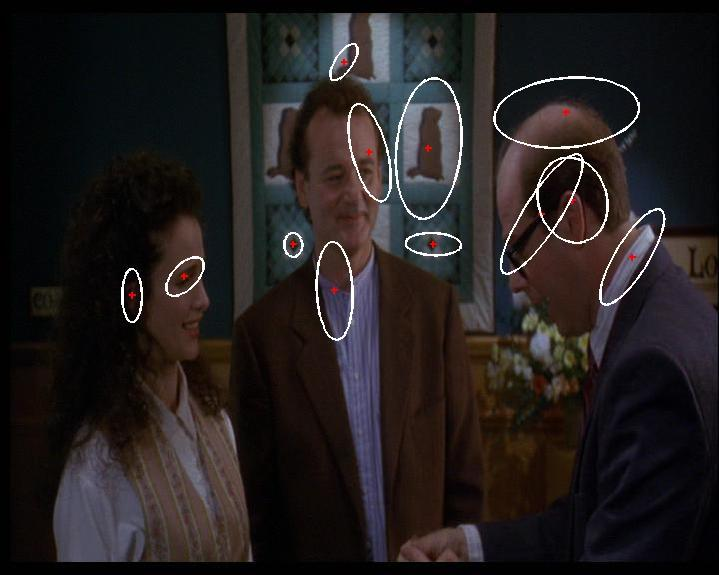
\includegraphics[width=0.5\textwidth]{FIGURES/groundhogday}~~
      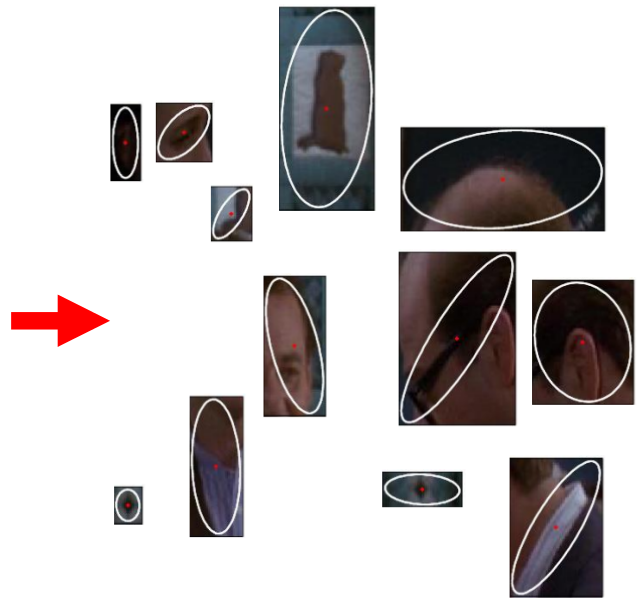
\includegraphics[width=0.5\textwidth]{FIGURES/gdwords}
    \end{center}
  \item Here patches centered around Harris Interest points.
  \item Other possibilities. Here we use SIFT descriptor (more than
    16000 citations means it must be interesting)
  \end{itemize}
\end{frame}


%-------------------------------------------------------------------
\begin{frame}
  \frametitle{Visual Words}
    \begin{itemize}
  \item Choose output from SIFT as building blocks for visual words.
  \item Produces generally 1000 -- 100.000 features per image.
    \begin{center}
      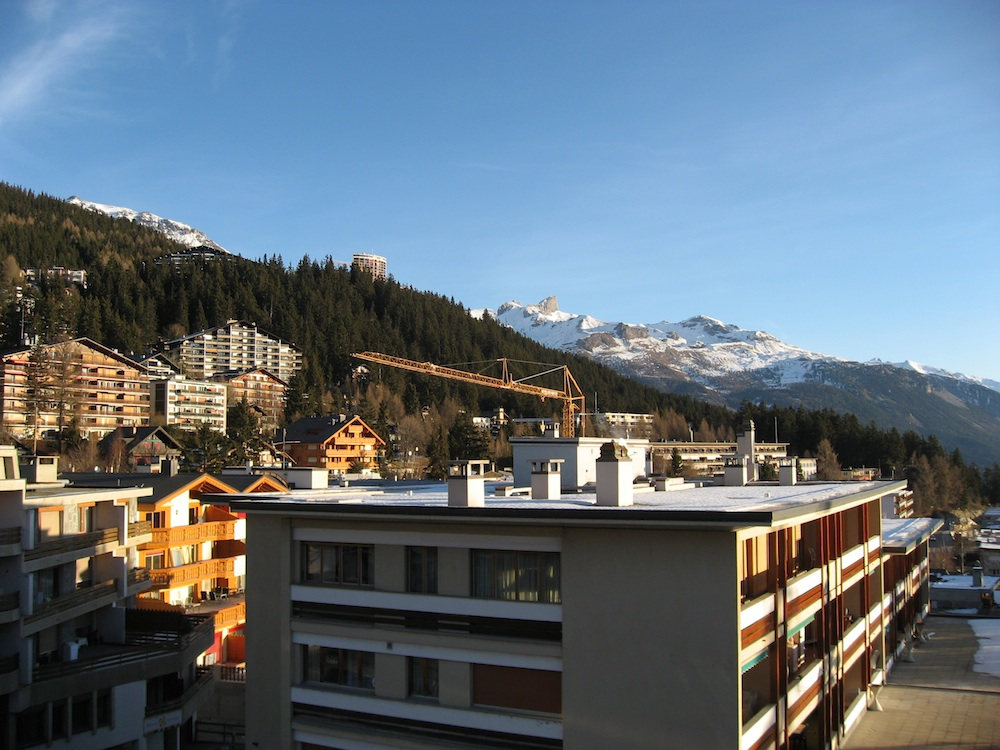
\includegraphics[width=0.4\textwidth]{FIGURES/crans_1_small}~~
      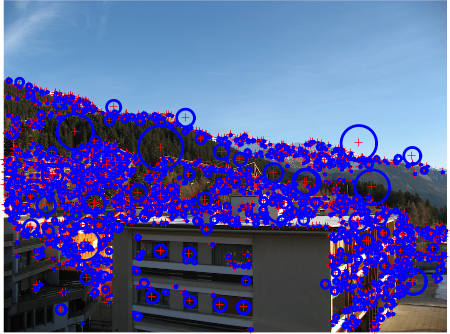
\includegraphics[width=0.4\textwidth]{FIGURES/cranswithsift}
    \end{center}
  \item Some are similar in content (as for text, e.g., ``Election / Electoral'')
  \item So group them by similarity.
  \end{itemize}
\end{frame}


%-------------------------------------------------------------------
\begin{frame}
\frametitle{What and how to sample}
  \begin{itemize}
  \item Points sampled in a grid
  \item Points detected as Blobs, Corners, Centers of symmetri, ...
  \item Areas: Segments, Objects (what is that?) \\[5mm]
  \end{itemize}

Which descriptors are best (most discriminative, yet robust/general)?
  \begin{itemize}
  \item Histograms of color, textons (texture elements) ?
  \item Coded spatial layout (eg. SIFT-like) ?
  \item ...
  \end{itemize}
\end{frame}


%-------------------------------------------------------------------
\begin{frame}
\frametitle{MPEG 7}
  \begin{itemize}
  \item Is a Multimedia Content Description Interface Standard \\[3mm]
  \item Defines a set of image and video descriptors including color
    descriptors, shape descriptors, motion descriptors etc. \\[3mm]
  \item Includes language for specifying the relations between
    descriptors and their spatial (or other) relationships. \\[3mm]
  \item Try Google {\color{blue}{MPEG 7 Standards}}. \\[3mm]
  \item There is much more to the story than you will learn here.
  \end{itemize}
\end{frame}


%-------------------------------------------------------------------
\begin{frame}
  \frametitle{Learning the Visual Words: Training}
  \begin{itemize}
  \item Collect all descriptor vectors from a training set of images 
    showing one class. They mush have something in common. \\[4mm]
  \item Group descriptors by similarity: clustering. \\[4mm]
  \item Choose prototypical representatives of each cluster: the \textbf{visual words}. \\[4mm]
  \item The set of visual words obtained is called \textbf{vocabulary} or \textbf{codebook}.
  \end{itemize}
\end{frame}


%\subsection{Clustering}
%\label{sec:clust}

%-------------------------------------------------------------------
\begin{frame}
  \frametitle{Clustering}
  \begin{definition}
    (from Wikipedia) Cluster analysis or clustering is the task of
    assigning a set of objects into groups (called clusters) so that
    the objects in the same cluster are more similar (in some sense
    or another) to each other than to those in other clusters.
  \end{definition}
  
  \vfill
  \begin{itemize}
  \item
    I will describe one standard technique for vector clustering: $K$-means clustering.
  \end{itemize}
\end{frame}


%-------------------------------------------------------------------
\begin{frame}
\frametitle{Good clustering}
{\color{red}{Exercise:}} \\
Discuss 2 minutes with your neighbor: What characterizes a good
clustering \\[5mm]
\pause

\begin{itemize}
  \item Small intra-cluster distances 
  \item Large inter-cluster distances 
\end{itemize}

Central for clustering is to have a good distance measure
\end{frame}


%-------------------------------------------------------------------
\begin{frame}
  \frametitle{A 2D Example}
  \begin{itemize}
  \item We want to cluster the following data
    \begin{center}
      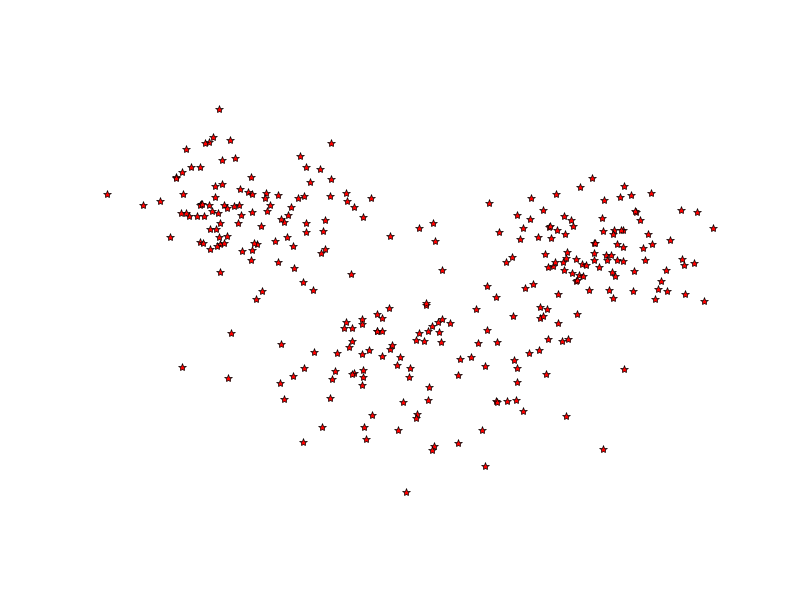
\includegraphics[width=0.8\textwidth]{FIGURES/2DData}
    \end{center}
  \item Visually 3 clusters.
  \end{itemize}
\end{frame}


%-------------------------------------------------------------------
\begin{frame}
  \frametitle{$K$-means Clustering}
  \begin{itemize}
  \item
    Given $n$ data vectors $x_1,\dots,x_n$ in $\RR^d$, find a
    \emph{partition} $\Ss$ of $\{1,\dots,n\}$ into $K$ subsets
    $S_1,\dots,S_K$, such that the \emph{Distortion} $\Dd$
    $$
    \Dd(S_1,\dots,S_K) = \sum_{i = 1}^K\sum_{j\in S_i} \|x_j -\mu_i\|^2
    $$
    is minimum, with
    $$
    \mu_i = \frac{1}{\#S_i}\sum_{j\in S_i}x_m = \text{mean of the }x_j, j\in S_i.
    $$
  \item The means become the prototypical representatives of the vectors, i.e., \textbf{the words}
  \end{itemize}
\end{frame}


%-------------------------------------------------------------------
\begin{frame}
  \frametitle{Standard Algorithm (Lloyd's Algorithm)}
  \begin{itemize}
  \item Choose  $K$ candidate cluster means $m_1,\dots,m_K$ (randomly).\vfill
  \item Then iterates the following two steps until no significant change occurs in the distortion $\Dd$\vfill
    \begin{enumerate}
    \item Assignment step: assign each observation $x_j$ to the cluster with closest mean $m_i$\vfill
    \item Update step: recompute the means of the clusters.\vfill
    \end{enumerate}
  \item {\color{red}{Exercise:}} Discuss for one minute with your
      neighbor: Does K-means always converge ?
  \end{itemize}
\end{frame}


%-------------------------------------------------------------------
\begin{frame}
  \begin{itemize}
   \item K-means always converge, but not necessarily fast nor to the
     right clustering. \\[4mm]
  \item To avoid local minima, run the {\em k-means} with different
    initial candidate clusters og choose the least bad one. \\[4mm]
  \item The distortion is specified by the sum of distances from
    each point to the nearest cluster (but there are other approaches). \\[4mm]
  \item You have to fix $K$.  There is no easy way to choose the
    optimal value. 
  \end{itemize}
\end{frame}


%-------------------------------------------------------------------
\begin{frame}
  \frametitle{2D example, $K = 3$}
  \begin{itemize}
  \item Run of $K$-means on the previous data.
    \begin{center}
      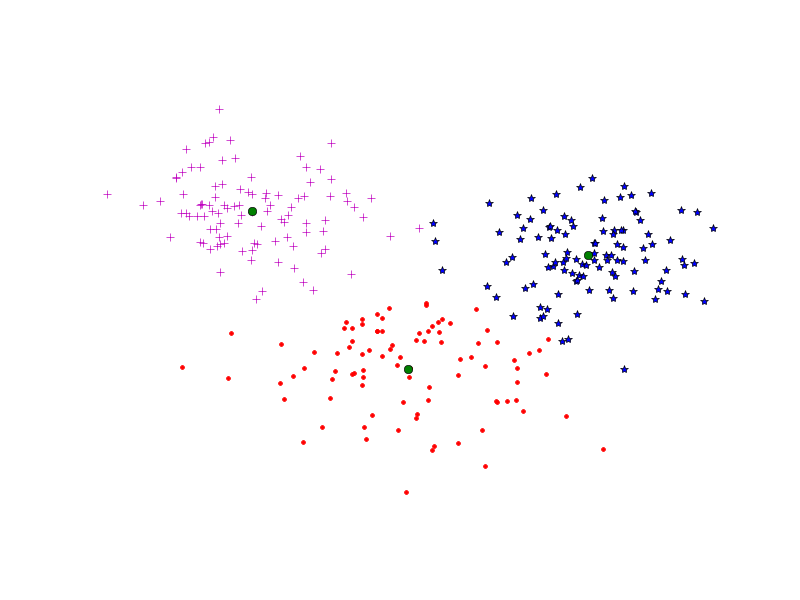
\includegraphics[width=0.8\textwidth]{FIGURES/2DData3Clusters}
    \end{center}
  \end{itemize}
\end{frame}


%-------------------------------------------------------------------
\begin{frame}
  \begin{itemize}
  \item Run with $K = 2$.
    \begin{center}
      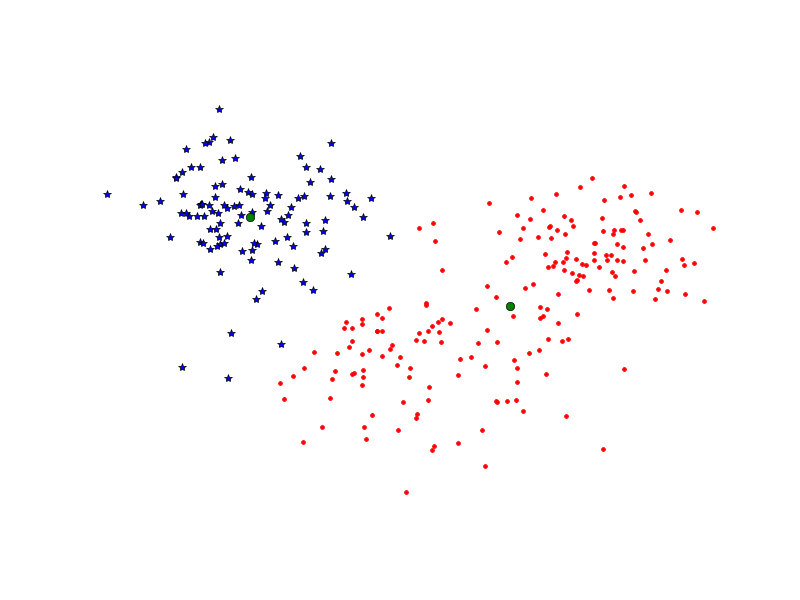
\includegraphics[width=0.8\textwidth]{FIGURES/2DData2Clusters}
    \end{center}
  \item $K$ can have a deep impact in the clustering results. 
  \end{itemize}
\end{frame}


%-------------------------------------------------------------------
\begin{frame}
  \frametitle{Other Clustering Methods}
  \begin{itemize}
  \item {\em Minimum Spanning tree}: Connect all points to its closest
    neighbor. Then iteratively remove the longest edge until left with
    $K$ clusters. \\[3mm]
  \item Hierarchical clustering: group data points by proximity,
    creates a binary tree-structure.  Each non-leaf node contains
    average distance between it subtrees. Clustering is performed by
    distance threshold. Number of clusters in not predefined. \\[3mm]
  \item Distribution model: observed data is produced by $K$
    distributions: clusters belong most likely to the same
    distribution, EM - {\em Expectation - Maximization}
    Algorithms. Can be very powerful. 
  \end{itemize}
\end{frame}


%-------------------------------------------------------------------
\begin{frame}
  \frametitle{Clustering and Words}
  \begin{center}
    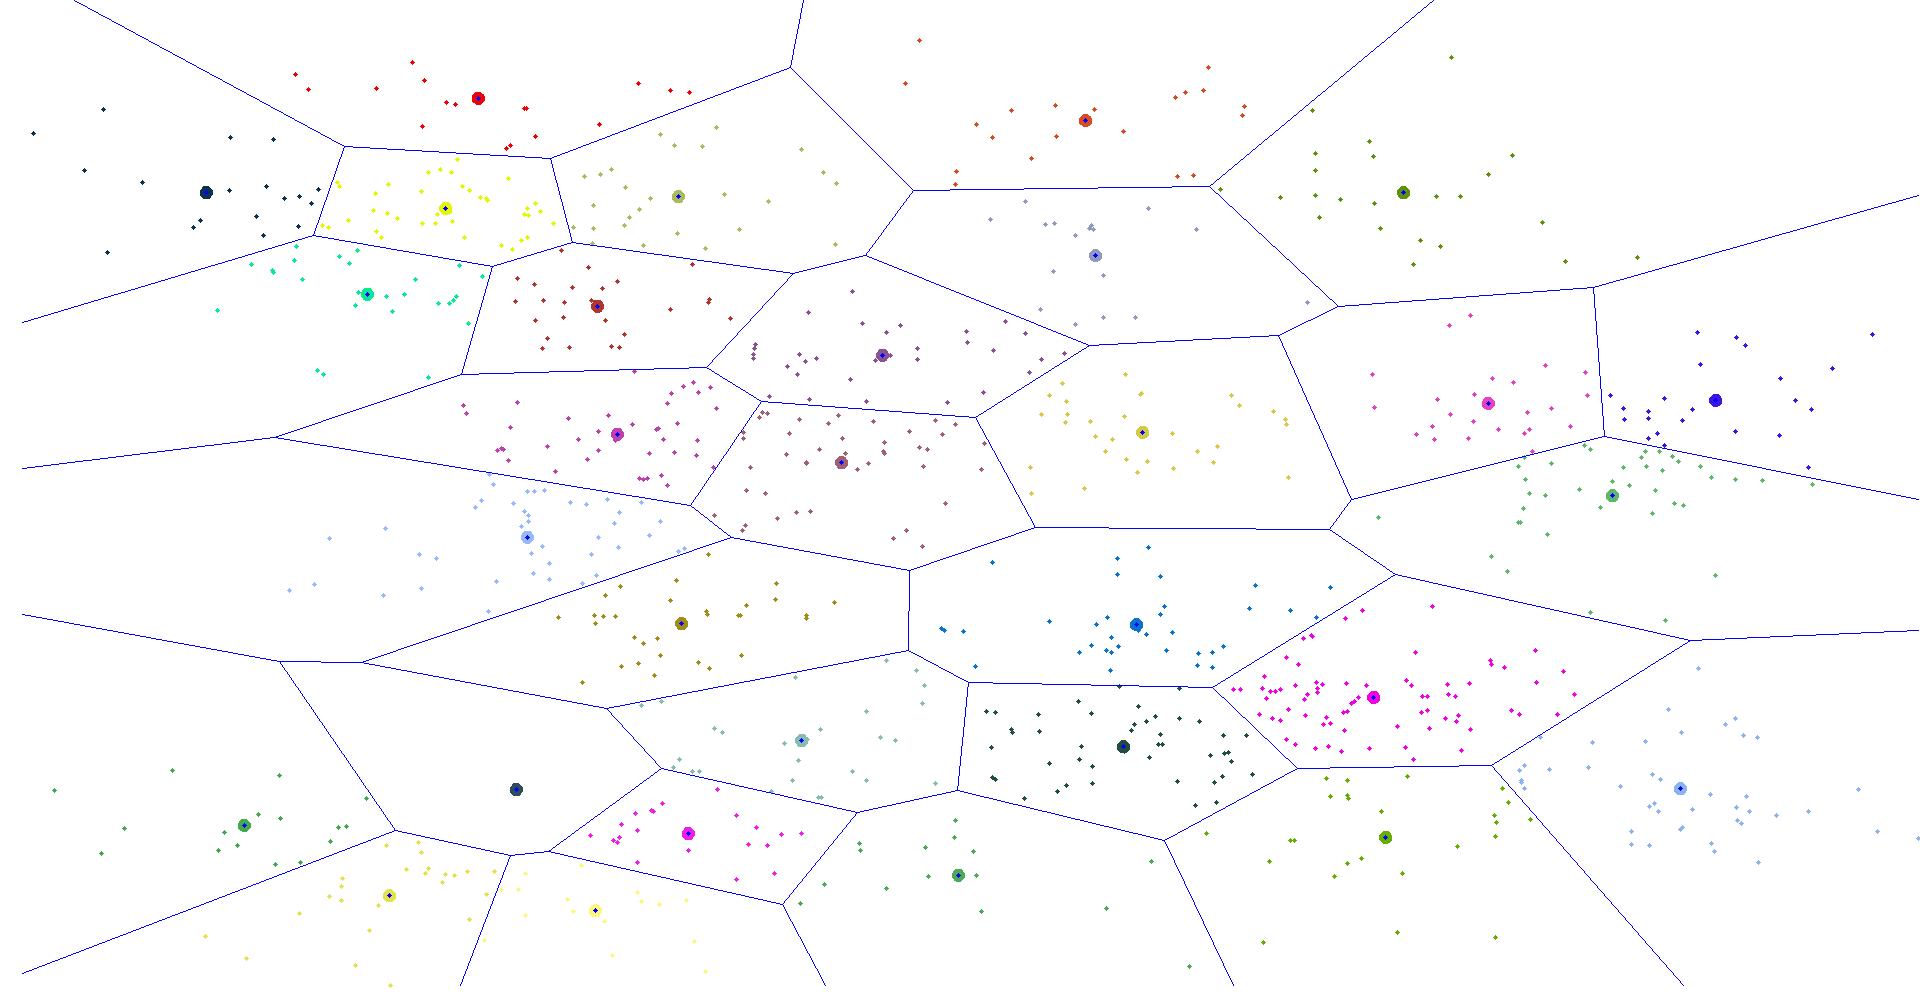
\includegraphics[width=0.6\textwidth, height=0.58\textheight]{FIGURES/clustervoronoi}
  \end{center}
  \begin{itemize}
  \item Words are cluster centers
  \item Each observation is assigned to the Voronoi cell it belongs to.
  \end{itemize}
\end{frame}


%-------------------------------------------------------------------
\begin{frame}
  \frametitle{Bag of Visual Words Representation of Images}
  \begin{itemize}
  \item Once the vocabulary is obtained, each image is ``projected'' to the vocabulary:
    \begin{enumerate}
    \item Compute descriptors for the image,
    \item Assign each of them to its closest word
    \item Count the number of occurrences of each word in the image. i.e.
      compute the histogram of the words for this image. 
    \end{enumerate}
  \item This histogram is the \textbf{Bag of words} (BOW) representation of
    the image.
  \item Spatial arrangement of the words is forgotten. Words are just ``thrown in a bag''.
  \item Histograms can be normalized. Each entry becomes the
    \textbf{word frequency} (or \textbf{term frequency}) in the image.
  \end{itemize}
\end{frame}


%-------------------------------------------------------------------
\begin{frame}
\frametitle{When do BOW malfunction}

{\color{red}{Exercise:}} \\
Discuss 2 minutes with your neighbor when a Bag of Words
representation is insufficient or misleading \\[4mm]
\pause

Example: When spatial arrangement do matter, eg. ``Putin on Obama''.
\pause
    \begin{center}
      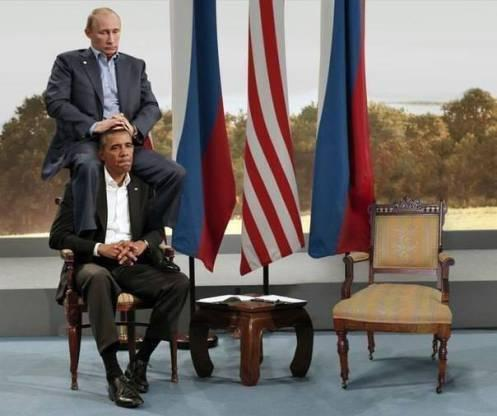
\includegraphics[width=0.5\textwidth]{MyImages/PutinOnObama.jpg}
    \end{center}
\end{frame}



\section{Similarity Measures}
\label{sec:simmeas}


%-------------------------------------------------------------------
\begin{frame}
  \frametitle{Ensemble of Common Words}
  \begin{itemize}
  \item Simple similarity measure: count the amount of common words between images \\[3mm]
  \item Can be used for query: return the images that have these ``words'' in common. \\[3mm]
  \item A subset of words can be used. %\\[3mm]
%   \item Easy to implement within a standard relational database. \\[3mm]
%   \item Discard bin sizes in histograms.
  \end{itemize}
\end{frame}


%-------------------------------------------------------------------
\begin{frame}
  \frametitle{Euclidean and Histogram Distances for BoVW}
  \begin{itemize}
  \item Euclidean Distance between two vectors 
    $$
    v_1 = \left(v_{11},\dots,v_{2K}\right), v_2 = \left(v_{21},\dots,v_{2K}\right), 
    d(v_1,v_2) = \sqrt{\sum_{i=1}^K\left(v_{1i}-v_{2i}\right)^2}
    $$
  \item Bhattacharyya Distance for Normalized Histograms:
    $$
    d(v_1,v_2) = \sum_{i=1}^K\sqrt{ v_{1i}\, v_{2i}}
    $$
  \item Kullback-Leibler Divergence for Normalized Histograms
    $$
    D_{KL}(v_1||v_2) = \sum_{i=1}^Kv_{1i}\,\ln\frac{v_{1i}}{v_{2i}}
    $$
    Not a distance as not symmetric, but can be symmetrized 
    $$
    d_{KL}\left(v_1,v_2\right) = \frac12\left( D_{KL}(v_1||v_2) +  D_{KL}(v_2||v_1)\right)
    $$
  \item $\chi^2$-distance measure $\sum \frac{|v_{1i} - v_{2i}|}{|v_{1i} + v_{2i}|}$
  \item {\em Earth movers distance}
  \end{itemize}
\end{frame}


%-------------------------------------------------------------------
\begin{frame}
  \frametitle{The Term Frequency -- Inverse Document Frequency }
  \begin{itemize}
  \item Some words (terms) are more common than other, not in one
    document but in a \textbf{corpus} (or data set). 
  \item Such terms are in general \textbf{less informative} (might be
    seen as a tautological statement!) 
  \item Inverse Document Frequency weighting reduces their importance:
    For a given word $w$ and a corpus $D$ 
    $$
    \idf_w = \frac{\# D}{\#\{d\in D, w\in d\}} 
    $$
    $\idf_w$ is a global weight.
  \end{itemize}
\end{frame}


%-------------------------------------------------------------------
\begin{frame}
  \begin{itemize}
  \item The \textbf{tf-idf} approach reweights the normalized histogram
    entries of document $d$ (the term frequencies) by the $idf$'s.
  \item Euclidean Distance or angle used as similarity. For a document
    $d$ in the data set and a query document $q$ 
    Compute the tf-idf reweighted BoVWs $v_d$ and $v_q$. 
  \item Define the similarity
    $$
    \text{sim}(d,q) = \text{angle}(v_d,v_q) = \arccos\frac{v_d\cdot v_q}{\|v_d\|\|v_q\|}
    $$
  \item In practice, the arc cosine is not computed. sim$(d,q)$ is the
    range [0,1], maximum similarity is 1. 
  \end{itemize}
\end{frame}


\section{Conclusion}


%-------------------------------------------------------------------
\begin{frame}
  \frametitle{Conclusion}
  \begin{itemize}
  \item We saw the major steps for a Content-Based Image Retrieval
    System based on the notion of learned vocabulary and bag of visual
    words.
  \item Step of training -- learning vocabulary
  \item Step of Indexing -- computing visual words
  \item Tools for searching / ranking -- computing similarity measures.
  \item Bag of Words is also used for object classification and recognition.
  \item Main Limitation is that BoVW ignores spatial relationships among the words
  \item Incorporating them is a hot research topic.
  \end{itemize}
\end{frame}

%-------------------------------------------------------------------
\begin{frame}
  \frametitle{Successful query?}
  \begin{center}
    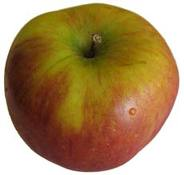
\includegraphics[width=0.2\textwidth]{FIGURES/anapple}\\
    
\includegraphics[width=0.05\textwidth]{FIGURES/redarrow}\\
    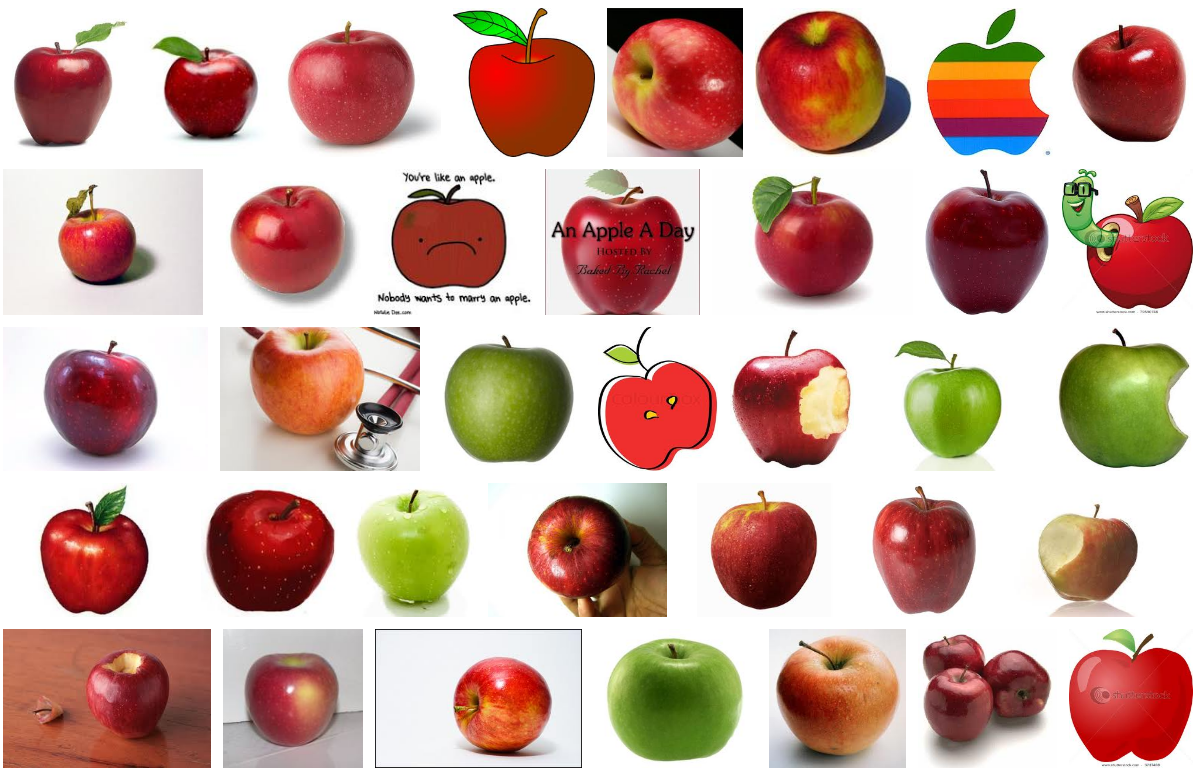
\includegraphics[width=0.6\textwidth]{FIGURES/applequery}\\
  \end{center}
\end{frame}


% \begin{frame}
%   \frametitle{A really smart CBIR system?}
%   \begin{center}
%    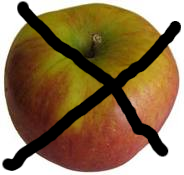
\includegraphics[width=0.2\textwidth]{FIGURES/noapple}\\
%    
\includegraphics[width=0.05\textwidth]{FIGURES/redarrow}\\
%    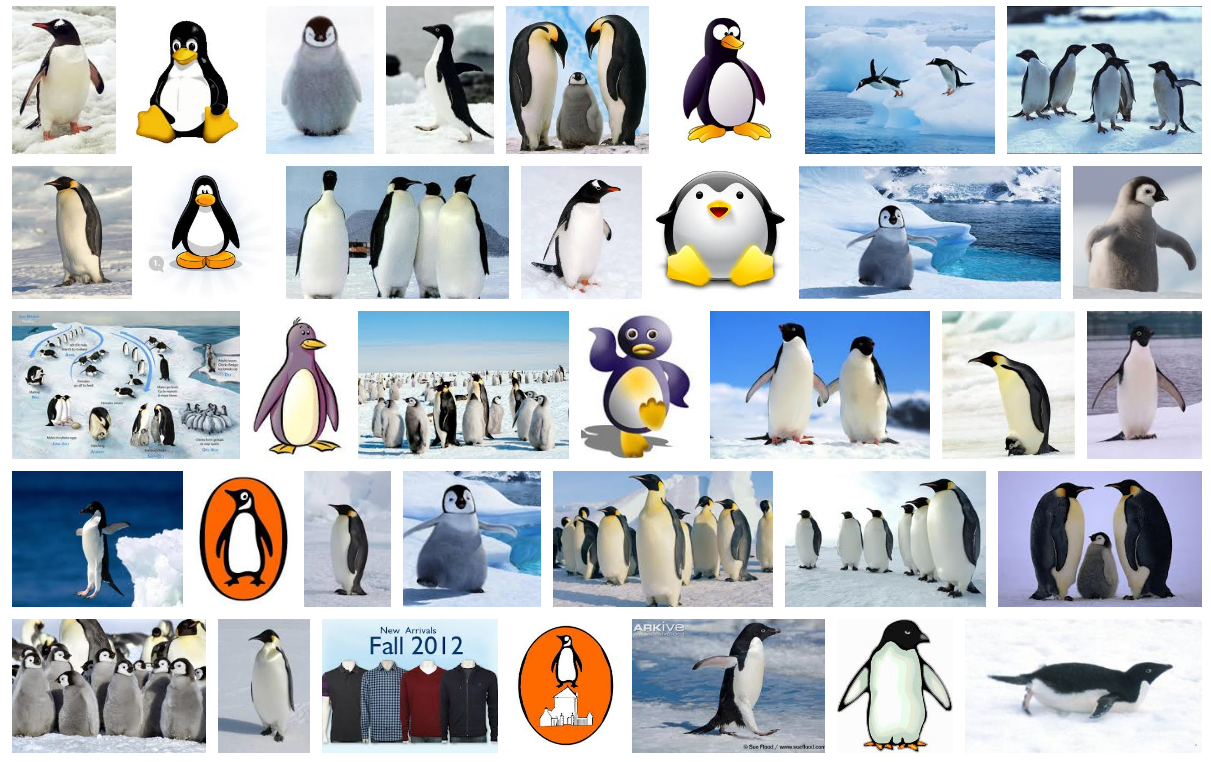
\includegraphics[width=0.6\textwidth]{FIGURES/Penguins}\\
%   \end{center}
% \end{frame}



\section{Assignment}
\label{sec:ass}


%-------------------------------------------------------------------
\begin{frame}
  \frametitle{Assignment}
  \begin{itemize}
  \item The assignment consists in implementing a prototypical Content
    Based Image Retrieval System \\[5mm]
  \item We'll discuss some details Wednesday. \\[5mm]
  \item Enjoy!
  \end{itemize}
\end{frame}


\end{document}
